
\chapter{Organization}

At the beginning of this internship I made many choices in the organization of my work.


\section{Calendar}

First of all, in June, I made a calendar of my planning works. This calendar has given me a good overview of the time that I am allow to spend in every task.



\begin{table}[h]
\noindent\begin{tabular*}{1\textwidth}{@{\extracolsep{\fill}} |c|*{14}{c|}}
\hline
  Tasks/weeks & 1 &2 &3&4&5&6&7&8&9&10&11&12&13&14\\
\hline
State of the art&-&-&&&&&&&&X&&&&\\
\hline
Create a plugin&&&-&&&&&&&X&&&&\\
\hline
Visualize the simulation&&&&-&-&-&-&-&&X&&&&\\
\hline
Unit tests&&&&&&&&-&&X&&&&\\
\hline
Integration tests&&&&&&&&&-&X&&&&\\
\hline
Try an other simulator&&&&&&&&&&X&-&-&&\\
\hline
Redaction&&-&-&-&-&-&-&-&-&X&-&-&-&\\
\hline
Oral&&&&&&-&&&&X&&&&-\\
\hline
\end{tabular*}
\caption{Calendar}
\end{table}


During the week 10, the University was closed, that is why it is a trivialized week.

\section{Record}

The main client of this project is Mr Champeau. So I did every week a record of my work by e-mail to him. In this e-mail I presented every week the work done during this week and the work planned for the next week. I put as much as possible a short video to present my improvements.

I also did a video conference with Mr Champeau and Mr Teodorov the 1th July. This video conference was very useful to know after 1 month if I take the good way and to clear some important point.




\section{Tools use for the project}

After the begin of this project I decided to use some tools to arrange my work.
~\\

I employ Framaboard. It is a web application which permit to create kanban board\footnote{Kanban is a method for managing knowledge used by software teams practicing agile software development.\cite{wiki_kanban}}. I used it because that allow to have a good visual overview of the project. The figure \ref{fig:framaboard} show my framaboard.

\begin{figure}[h]
  \centering
  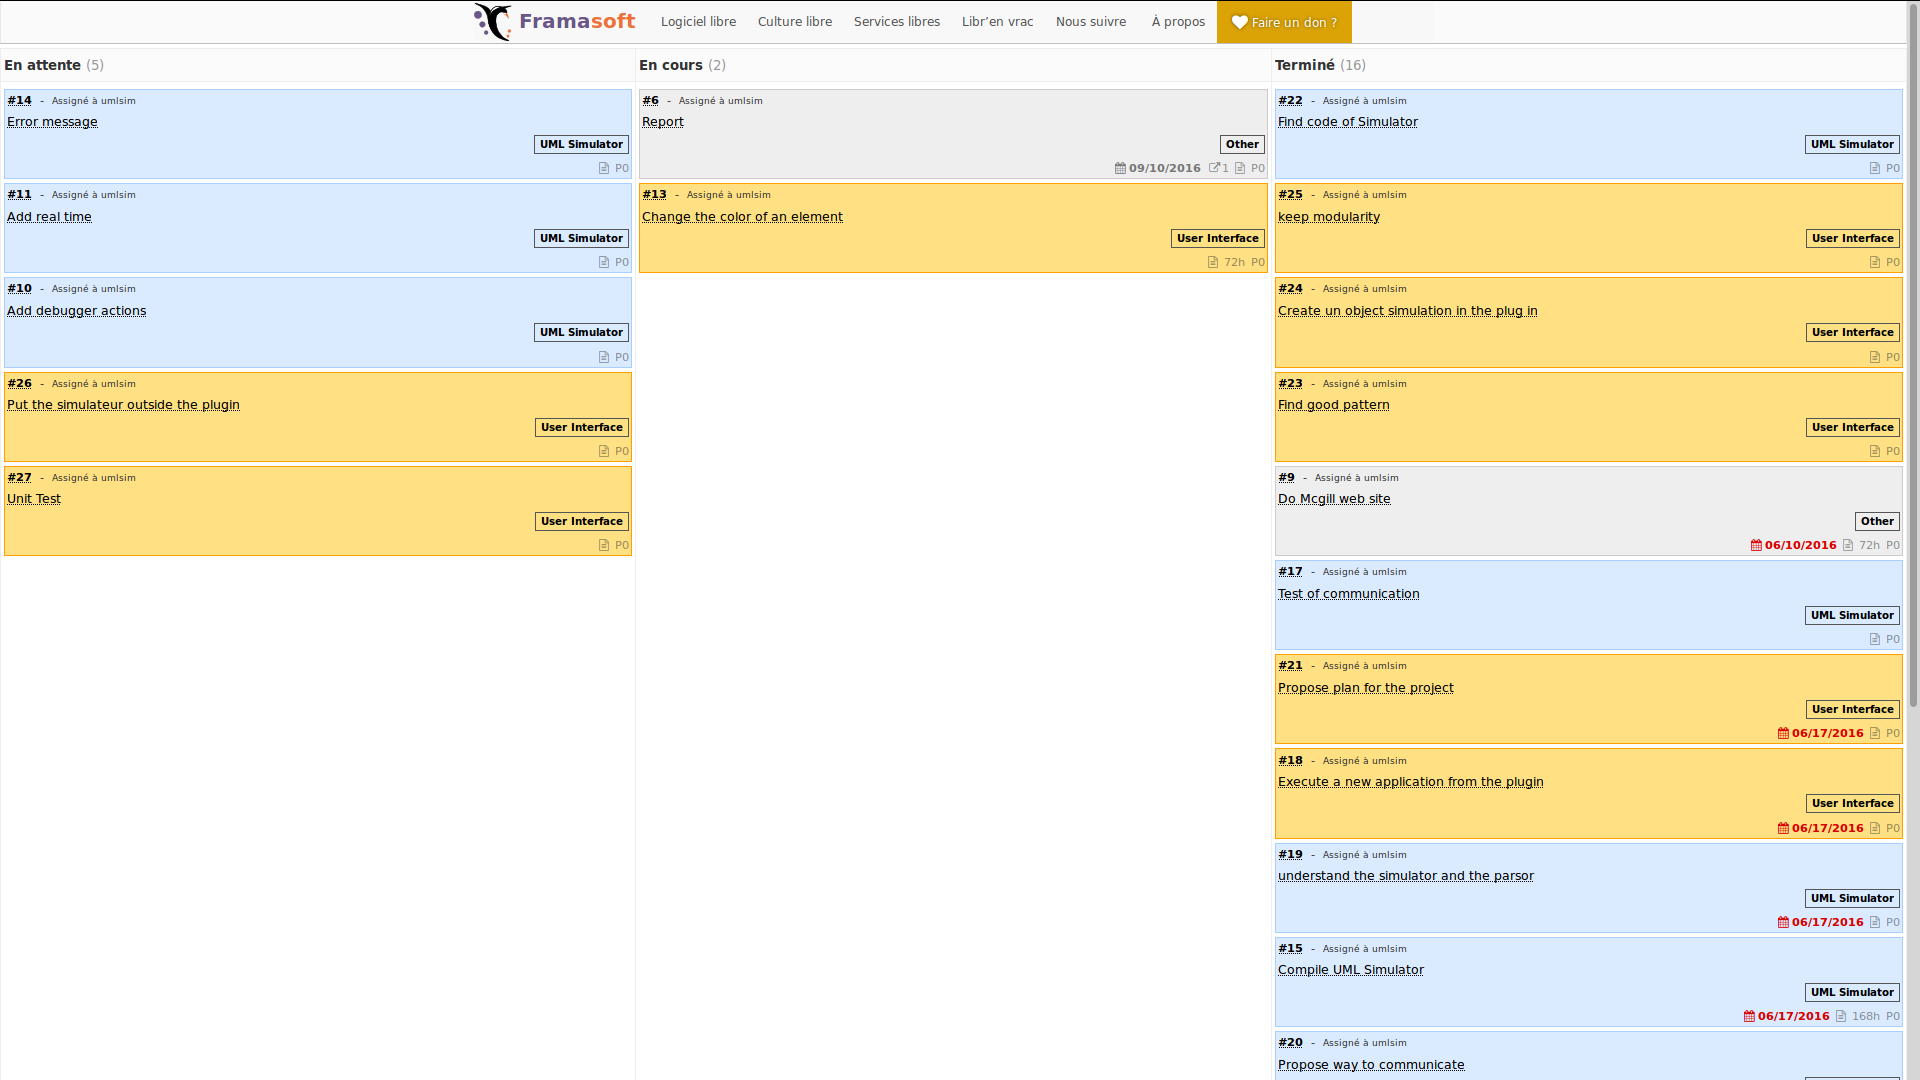
\includegraphics[width=\textwidth]{framaboard}
  \caption{Screen shot of the framaboard}
  \label{fig:framaboard}
\end{figure}

Then the MSDL laboratory give me a web page to present my work and my progress. I also put on this web page a resume of all my records. The figure \ref{fig:msdl} exhibit my personal web page.

\begin{figure}[h]
  \centering
  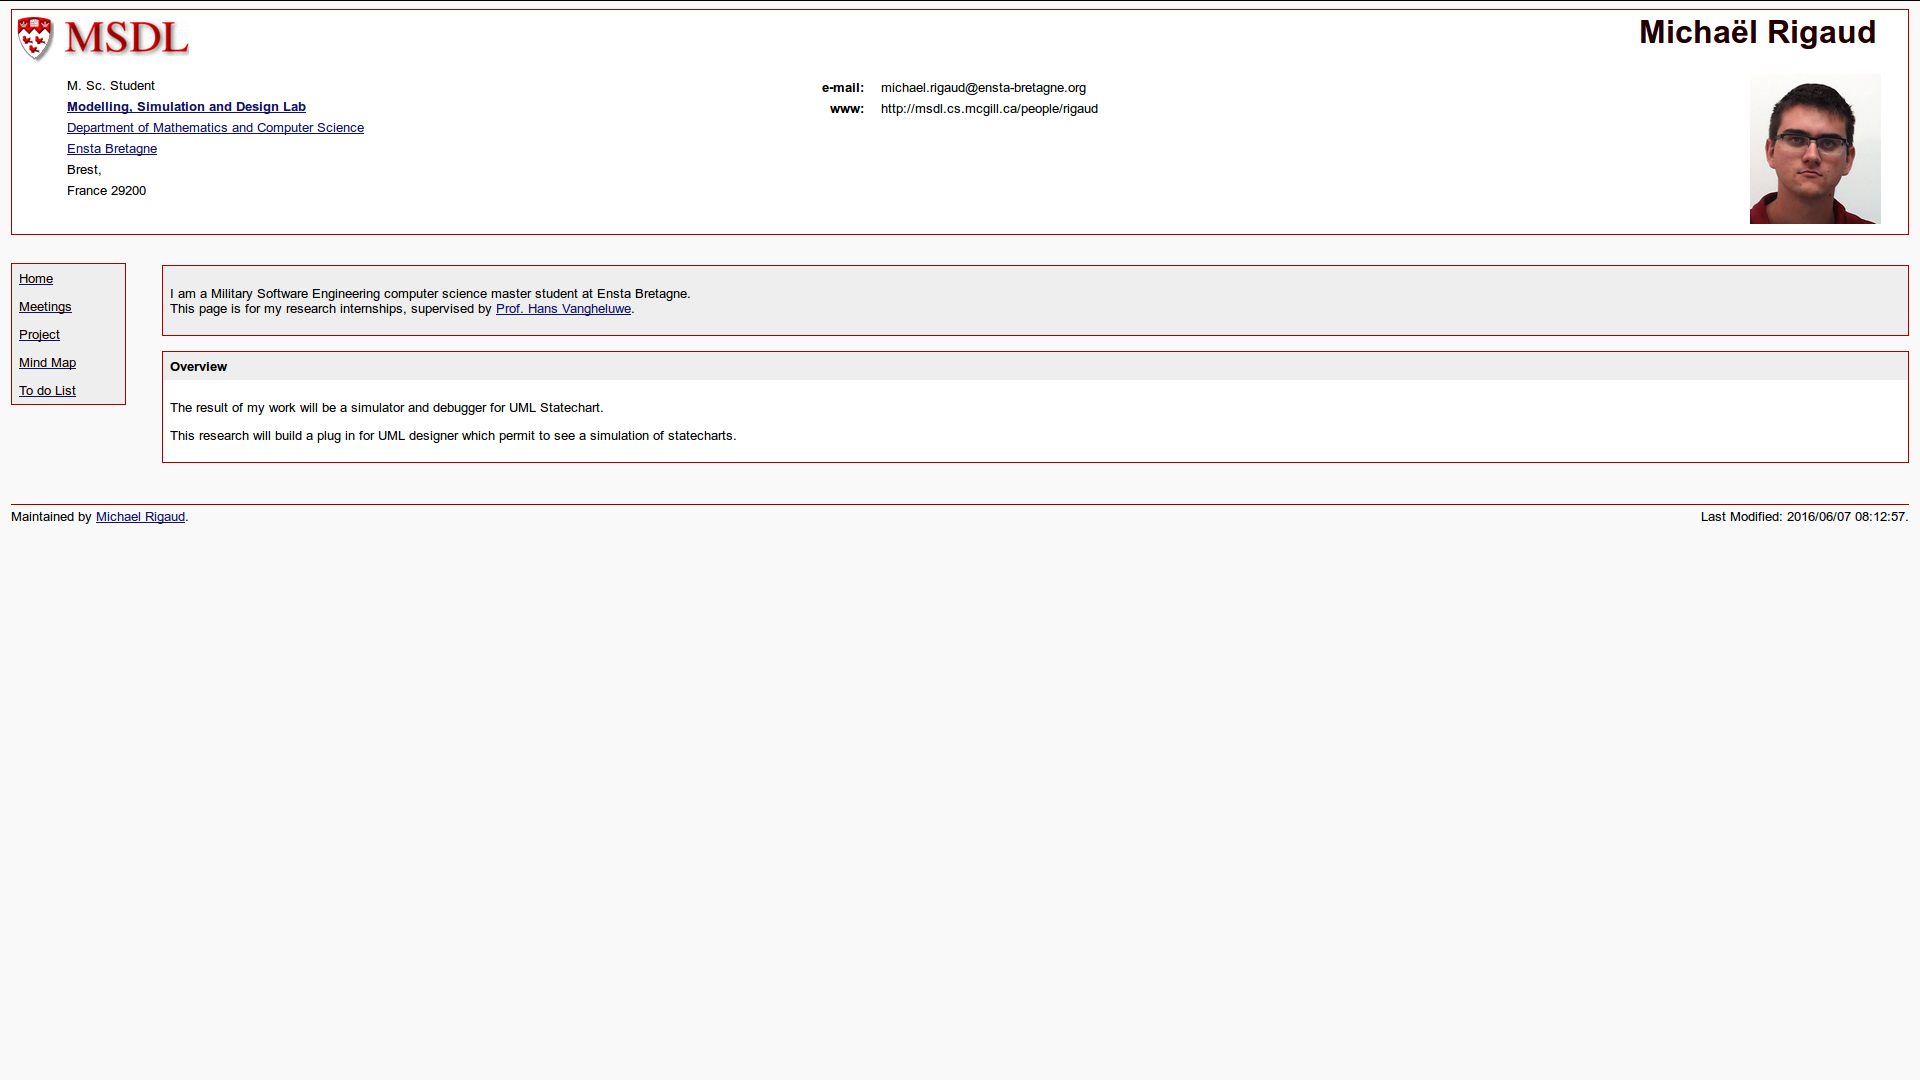
\includegraphics[width=\textwidth]{msdl}
  \caption{MSDL web site}
  \label{fig:msdl}
\end{figure}


To finish they likewise give me an access to their git server. That permit to lodge my work on a secure server and prevent a breakdown of my computer. The figure \ref{fig:git} show my git repository.

\begin{figure}[h]
  \centering
  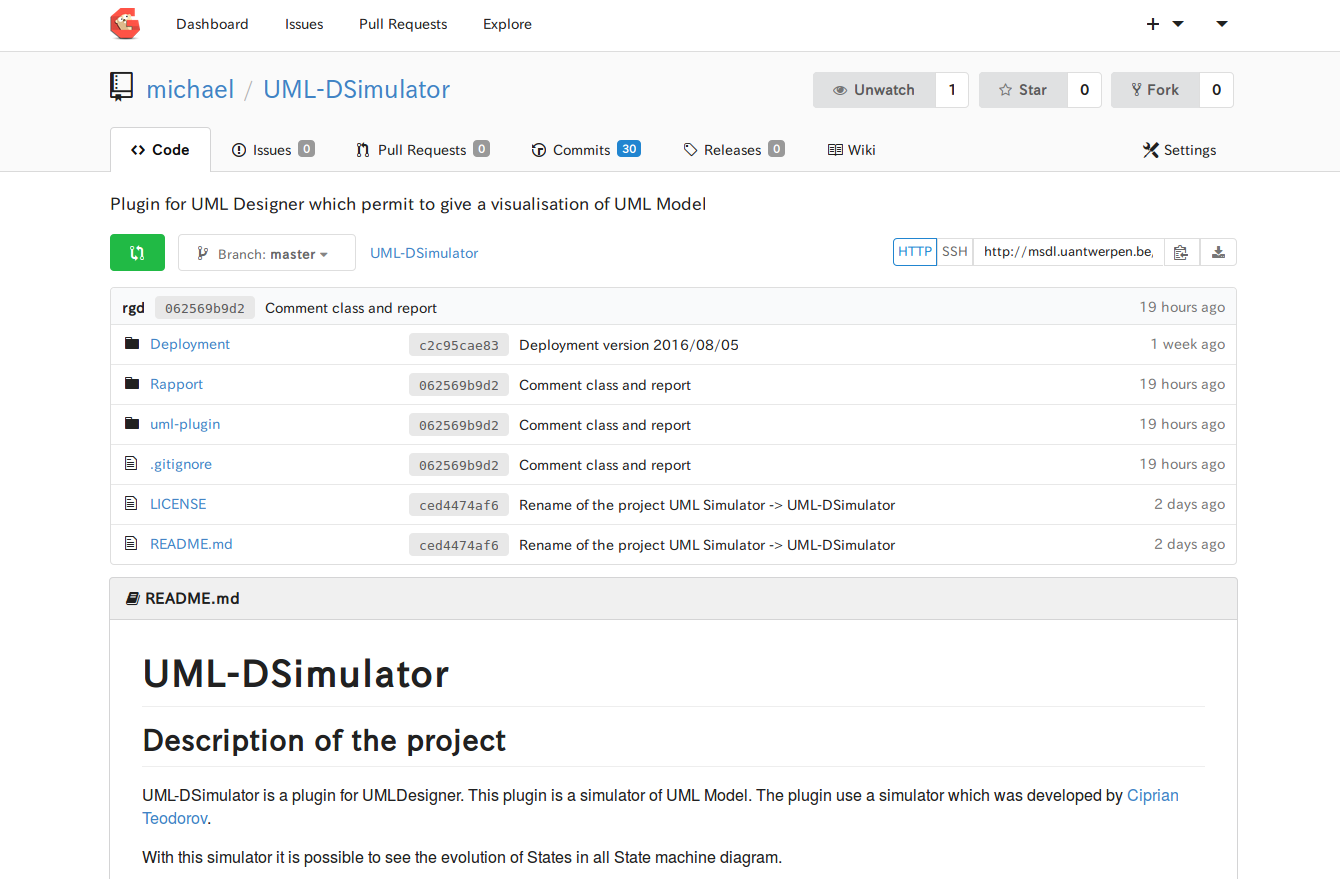
\includegraphics[width=\textwidth]{git.png}
  \caption{git repository}
  \label{fig:git}
\end{figure}



%%% Local Variables:
%%% mode: latex
%%% TeX-master: "../rapport_de_base"
%%% End:
